\section{Accounts and Enrollments}

\subsection{Login and Sign Up}
\textbf{Functional and Non-Functional Requirements}

The requirements laid out in the project plan for the login and sign up feature were as follows:
    \begin{enumerate}
    \item Users can register and login \textcolor{Red}{High}
    \item administrators can create accounts on behalf of students \textcolor{Blue}{Low}
    \end{enumerate}
The first requirement was achieved very early in the project as it was high priority, while the second was not completed as part of the Thesis, however will be listed to be completed in future work. It not completed due to the prioritisation of other advanced features such as the login code invite redirect causing this feature to be demoted in priority.

\textbf{Usability Tests}

There was one usability test conducted in relation to this feature. Three students and one teacher completed this and all the remainder of the tests for the accounts and enrollment feature.

\begin{table}[h!]
\centering
\begin{tabular}{|l|l|}
\hline
\textbf{Login and Sign up - Task 1}     & \textbf{Description}                                                                                                                                          \\ \hline
\textit{Task}                           & Register for an account and sign in                                                                                                                           \\ \hline
\textit{Starting State}                 & The login page                                                                                                                                                \\ \hline
\textit{Successful Completion Criteria} & \begin{tabular}[c]{@{}l@{}}- Navigated to the sign up form from the login page\\ - Correctly fills all fields\\ - Submits the form once complete\end{tabular} \\ \hline
\textit{Benchmark}                      & 30 seconds                                                                                                                                                    \\ \hline
\end{tabular}
\end{table}

All four of the users were able to very easily complete this test within the allotted time. This can be attributed to the simple design that is comparable to other login and sign up flows that exist elsewhere on the internet.

\textbf{Performance and Accessibility}

Google Lighthouse was used to benchmark the performance and accessibility of all of the features within accounts and enrollments. Google lighthouse uses automated tests to asses the response time of the page, and then analyses the code executed to build the page to find what may be causing a page to take a long time to respond and render. It also uses this same analysis to determine whether best accessibility practices have been used such as using appropriate alt-tags and aria labels where possible, and ensuring that components have proper contrast.

\begin{figure}[h!]
    \centering
    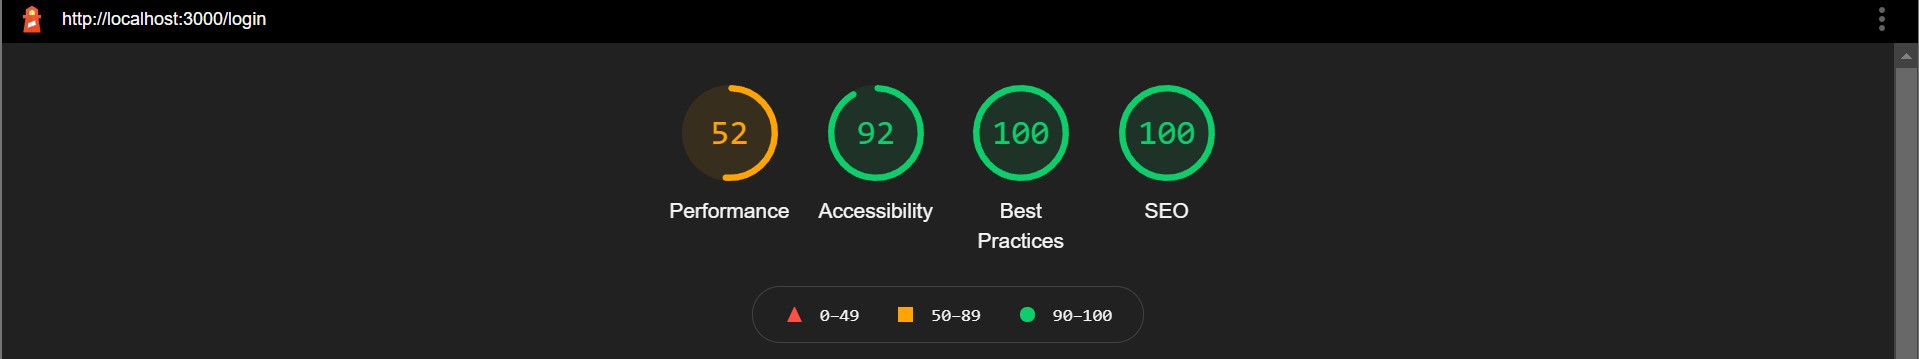
\includegraphics[scale=0.3]{images/accounts-login-lighthouse.jpg}
    \caption{Google Lighthouse Results for the Login and Sign Up Page}
\end{figure}

The login page scored a 52/100 for performance and a 92/100 for accessibility. The performance score is primarily due to the non-minified state of the JavaScript. Minifying JavaScript is a process whereby the files that make up a web-page are processed to reduce file size by removing white-space and reducing all the code down to one line. As the Meta LMS is still in development, minifying the JavaScript is not feasible, as it makes the code for the site non-human readable and thus non-editable. The other performance impact is unused JavaScript.

The accessibility score was not a perfect 100 due to a HTML container that is used to control the spacing on the page having an incorrect aria label. This can cause users with screen readers to have a hard time navigating the web page, however this can be easily remedied by refactoring the page's code.

\textbf{Timeline}

From the timeline set out in the project plan, the login and sign up feature was planned to be finished by week 4 of term 2. The front-end component of this feature was completed by this time, however the back-end component of this feature took an additional 6 weeks to finish. The reasons for which will be discussed in the following challenges section.

\textbf{Challenges Faced}

The extended timeline for completing the login and sign up feature was due to unforeseen complexities that resulted from developing authentication features in parallel with the rest of the LMS, meaning that the ever changing specification of the other features caused the nature of the authentication process to need to change a number of times through development. This could have been resolved by developing authentication before any of the other features, however this would have caused delays for the other portions of the LMS.


\subsection{Account Management}
\textbf{Functional and Non-Functional Requirements}

The requirements laid out in the project plan for the login and sign up feature were as follows:
    \begin{enumerate}
    \item Users can view and update their details \textcolor{Red}{High}
    \item administrators can manage users, roles and permissions \textcolor{Blue}{Low}
    \item administrators can view other users account details \textcolor{Blue}{Low}
    \end{enumerate}
The first requirement was successfully achieved, however the second two were lowered in priority in favor of advanced enrollment features and were subsequently not completed. However, the current accounts system was developed with these features in mind, and it is very feasible for the current system to be updated to support this functionality with future work. 

\textbf{Usability Tests}

There was two usability tests conducted in relation to this feature. Three students and one teacher completed them.
\begin{table}[h!]
\centering
\begin{tabular}{|l|l|}
\hline
\textbf{Account Management - Task 1}    & \textbf{Description}                                                                                                                                                                                                                           \\ \hline
\textit{Task}                           & Change your email                                                                                                                                                                                                                              \\ \hline
\textit{Starting State}                 & The Site Dashboard                                                                                                                                                                                                                             \\ \hline
\textit{Successful Completion Criteria} & \begin{tabular}[c]{@{}l@{}}- Navigated to the account management screen from\\the dashboard\\ - Sets the account management page to edit mode\\ - Fills in the new email and current password\\ - Successfully submits the changes\end{tabular} \\ \hline
\textit{Benchmark}                      & 90 seconds                                                                                                                                                                                                                                     \\ \hline
\end{tabular}
\end{table}

\begin{table}[h!]
\centering
\begin{tabular}{|l|l|}
\hline
\textbf{Account Management - Task 2}    & \textbf{Description}                                                                                                                                                                                                  \\ \hline
\textit{Task}                           & Change your password                                                                                                                                                                                                  \\ \hline
\textit{Starting State}                 & The account management page                                                                                                                                                                                           \\ \hline
\textit{Successful Completion Criteria} & \begin{tabular}[c]{@{}l@{}}- Sets the account management page to edit mode\\ - Fills in the new password and confirm password fields\\ - Enters current password\\ - Successfully submits the changes\end{tabular} \\ \hline
\textit{Benchmark}                      & 90 seconds                                                                                                                                                                                                            \\ \hline
\end{tabular}
\end{table}
The purpose of test 1 was to determine whether users were easily able to find the account management page and then decipher the editing system. All 4 of the participants managed to successfully find the accounts page with no additional help, however one took considerably longer to find the drop-down menu on the dashboard. This can be attributed to the lack of an indication that clicking on the users name and image in the top right will display a drop-down menu, which can be rectified by adding a down arrow icon next to the text, or an underline to the text to indicate its clickable. Once on the account page, all users very quickly found the edit button and filled the email field. 3 of the 4 participants tried submitting the form without confirming their password which resulted in an error. All of the participants successfully completed the task, but 2 of the 4 did not finish within the benchmark time, due to not finding the drop-down and missing the confirm password portion of the form. The confirm password issue could be resolved with more visibility to the required nature of that field for the form, perhaps by adding a subheading above that input, as the current implementation of the red asterisks next to the text fields label was easily overlooked by participants.

The second test was completed much more successfully by all participants. After having already used the edit feature, all participants correctly filled the form to change both fields, remembering to confirm their own password, and intrinsically understanding to confirm their new password before submitting. This speaks to the learn-ability of the account management feature.

\textbf{Performance and Accessibility}

\begin{figure}[h!]
    \centering
    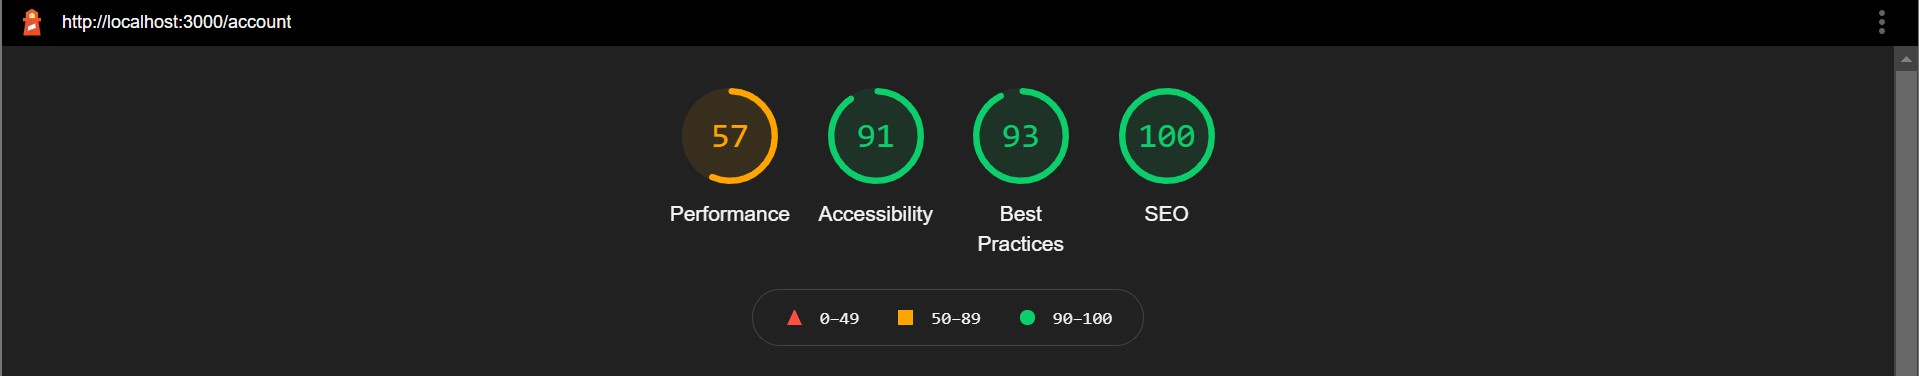
\includegraphics[scale=0.3]{images/accounts-accounts-lighthouse.jpg}
    \caption{Google Lighthouse Results for the Account Management Page}
\end{figure}
The accounts page received near identical scores to the login and sign up page, with the same criticisms for each of the criteria. The accessibility score was a 91/100 due to some divs in the page that were used for styling not having the correct aria labels, and the performance was mostly impacted by non-minified JavaScript. Both of these can be easily rectified.

\textbf{Timeline}

The timeline originally defined when planning was that users would be able to view their account information by Week 6 Term 2, and edit it by Week 4 Term 3. However, both of these features were delayed to being worked on from between Week 2 Term 3 and Week 5 Term 3. This was done to ensure that the enrollment features that were more essential to the functionality of the LMS as a whole being were completed first.

\textbf{Challenges Faced}

One of the primary challenges faced while developing this feature was the ability to add profile images. We did not want to store these images within the database, as that would increase the size of any payloads containing these images to be extremely large, causing the entire site to slow down, but we did not have the time or resources to develop a separate online storage for these images within the project. Thus, as a temporary measure, users are able to enter a link to an image to be used as their profile image. This is not a good solution from a user experience perspective, but it is functional for the time being. However, due to the nature of the current system pointing to a URL that stores an image, future work can be done to quite easily add an online store for images once more resources to fund online storage are available.

\subsection{Enrollment Dashboard - Staff}
\textbf{Functional and Non-Functional Requirements}

The requirements laid out in the project plan for the staff enrollment dashboard feature were as follows:
    \begin{enumerate}
    \item administrators can enrol and un-enroll students on their behalf \textcolor{Red}{High}
    \item administrators can generate course invite codes \textcolor{Red}{High}
    \item administrators can set courses to be open enrolment or invite/code only \textcolor{Red}{High}
    \item administrators can open and close enrolments for courses \textcolor{Orange}{Medium}
    \end{enumerate}
All 4 of these requirements were successfully completed. They were all made high priority once development commenced due to the importance of them to the functioning of the broader LMS.

\textbf{Usability Tests}

There were three usability tests conducted in relation to this feature. One teacher completed them.

\begin{table}[h!]
\centering
\begin{tabular}{|l|l|}
\hline
\textbf{Staff Enrollment Dashboard - Task 1} & \textbf{Description}                                                                                                                                                                                                                   \\ \hline
\textit{Task}                                & \begin{tabular}[c]{@{}l@{}}Delete an existing invite code and generate a new one with\\ limited uses, then copy it to the clipboard\end{tabular}                                                                                       \\ \hline
\textit{Starting State}                      & A course's dashboard                                                                                                                                                                                                                   \\ \hline
\textit{Successful Completion Criteria}      & \begin{tabular}[c]{@{}l@{}}- Navigates to the enrollment dashboard\\ - Identifies the code to delete and deletes it\\ - Sets the number of uses for the new code\\ - Generates the new code and saves it to the clipboard\end{tabular} \\ \hline
\textit{Benchmark}                           & 60 seconds                                                                                                                                                                                                                             \\ \hline
\end{tabular}
\end{table}

\begin{table}[h!]
\centering
\begin{tabular}{|l|l|}
\hline
\textbf{Staff Enrollment Dashboard - Task 2} & \textbf{Description}                                                                                           \\ \hline
\textit{Task}                                & Set the state of the course to search-able                                                                      \\ \hline
\textit{Starting State}                      & A course's enrollment dashboard                                                                                \\ \hline
\textit{Successful Completion Criteria}      & \begin{tabular}[c]{@{}l@{}}- Identifies the search-ability toggle\\ - Set the course to search-able\end{tabular} \\ \hline
\textit{Benchmark}                           & 10 seconds                                                                                                     \\ \hline
\end{tabular}
\end{table}

\begin{table}[h!]
\centering
\begin{tabular}{|l|l|}
\hline
\textbf{Staff Enrollment Dashboard - Task 3} & \textbf{Description}                                                                                                                                                                                    \\ \hline
\textit{Task}                                & Manually enroll a student, un-enroll that student                                                                                                                                                        \\ \hline
\textit{Starting State}                      & A course's enrollment dashboard                                                                                                                                                                         \\ \hline
\textit{Successful Completion Criteria}      & \begin{tabular}[c]{@{}l@{}}- Identifies the manual enrollment box and enters a\\ students ID\\ - Identifies that same student in the student list\\ - Successfully un-enrolls that student\end{tabular} \\ \hline
\textit{Benchmark}                           & 60 seconds                                                                                                                                                                                              \\ \hline
\end{tabular}
\end{table}

Each of the tests were designed to test one of the three key enrollment features. Task 1 focuses on the invite code feature. The participant was easily able to navigate to the enrollment dashboard, and found the code to delete very quickly. They also very quickly identified the delete button and successfully deleted the code. They took a little while to analyse the code generation form and read the sub-headings, but generated the new code and copied it to clipboard with no difficulty. An interesting note was that they used the copy button from within the table list rather than the one at the top of the page next to the code. When asked why, they responded by saying that they did not realise the top one was there. This can be addressed by increasing the size of that button and perhaps making it a more visible color.

Task 2 was completed very quickly. After a cursory screening of the page, the participant found and toggled the search-ability switch well within the benchmark time. Task 3 was also completed with ease, the participant very quickly found the text input, enrolled the student with the given ID, and were able to easily find the student with the corresponding student ID that was just enrolled, and used the un-enroll button to un-enroll them well within the benchmark time. A comment the participant made was that when they have a larger course size, it may be more difficult to find a student in the student list, and suggested perhaps a search bar or more advanced filtering for the student list.


\textbf{Performance and Accessibility}

\begin{figure}[h!]
    \centering
    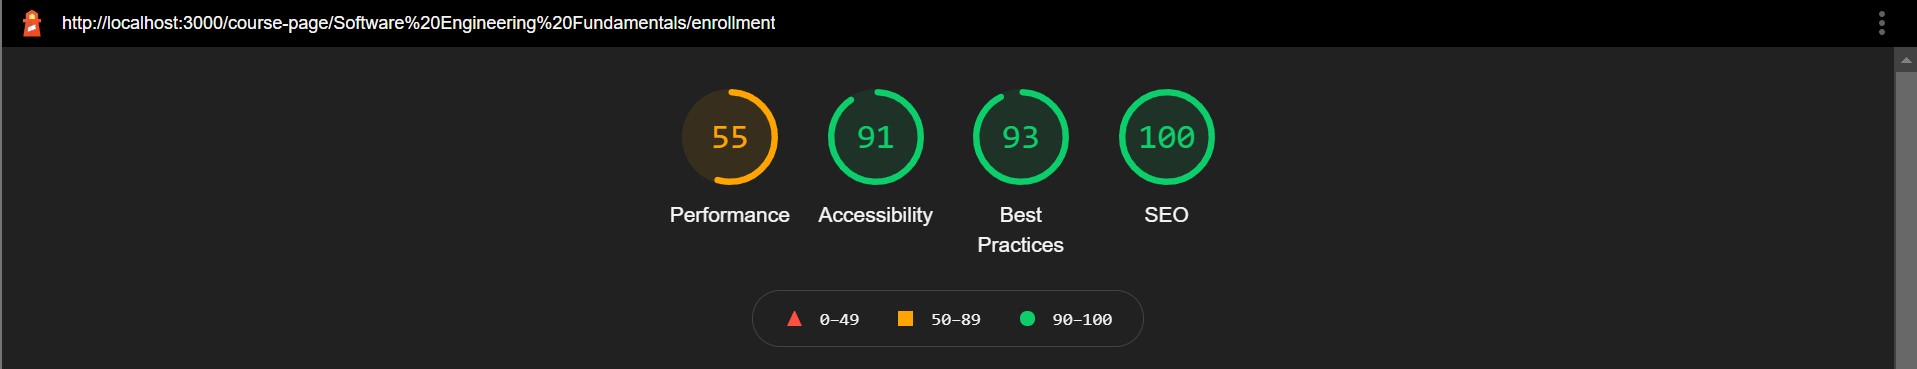
\includegraphics[scale=0.3]{images/accounts-staff-lighthouse.jpg}
    \caption{Google Lighthouse Results for the Staff Enrollment Dashboard}
\end{figure}

The staff enrollment dashboard received near identical scores to the login and sign up page, with the same criticisms for each of the criteria. The accessibility score was a 91/100 due to some divs in the page that were used for styling not having the correct aria labels, and the performance was mostly impacted by non-minified JavaScript. Both of these can be easily rectified.

\textbf{Timeline}

In the original timeline, this was broken out into standard and advanced enrollment features, with the standard features being manual enrollment and advanced being everything else. Standard features were planned on being completed in Week 9 of Term 2, and was completed on schedule. Advanced features were planned on being finished in Week 4 of Term 3, by which the code enrollment was completed, but the search functionality wasn't completed until week 7.

\textbf{Challenges Faced}

This feature contained the bulk of the feature work for the accounts and enrollment feature, due to the fact that a lot of the back-end architecture for the student enrollment features had to be considered and developed as a part of the staff enrollment features. As a result, many decisions had to be made regarding the structure of the database, and how student and staff accounts would interact with entries for courses and topics. The eventual decision was to create a new table that contained the course id, the user id, the date enrolled and the users progress through the course to represent an enrollment. This format gives us the flexibility to be able to search enrollments per user, and per course, as well as gain some basic information about these enrollments very easily.

Another challenge faced was the architecture for the invite code feature. It became difficult to ensure that none of the codes in the database were expired, leading to potential misleading information on the enrollment dashboard and potential erroneous enrollments. To combat this, every time an enrollment code is accessed, its validity is checked, and also, while the staff enrollment dashboard is open, the invite code table is reloaded every 5 minutes to force the back-end to check the validity of all the enroll codes and to give the front-end the most up to date information about the number of uses and time remaining for each of these codes.

\subsection{Enrollment Dashboard - Student}
\textbf{Functional and Non-Functional Requirements}

The requirements laid out in the project plan for the student enrollment dashboard feature were as follows:
    \begin{enumerate}
    \item Students can enrol themselves in courses with a code \textcolor{Red}{High}
    \item Students can search for open courses \textcolor{Red}{High}
    \item Students can enrol themselves in an open course or topic \textcolor{Red}{High}
    \end{enumerate}
All 3 of these requirements were successfully completed. They were all made high priority once development commenced due to the importance of them to the functioning of the broader LMS.

\textbf{Usability Tests}

There were three usability tests conducted in relation to this feature. Three students completed them.

\begin{table}[h!]
\centering
\begin{tabular}{|l|l|}
\hline
\textbf{Student Enrollment Dashboard - Task 1} & \textbf{Description}                                                                                                                                  \\ \hline
\textit{Task}                                  & Enroll with an invite code                                                                                                                            \\ \hline
\textit{Starting State}                        & Site dashboard                                                                                                                                        \\ \hline
\textit{Successful Completion Criteria}        & \begin{tabular}[c]{@{}l@{}}- Correctly navigates to the student enrollment\\dashboard\\ - Enters the invite code and successfully enrolls\end{tabular} \\ \hline
\textit{Benchmark}                             & 60 seconds                                                                                                                                            \\ \hline
\end{tabular}
\end{table}

\begin{table}[h!]
\centering
\begin{tabular}{|l|l|}
\hline
\textbf{Student Enrollment Dashboard - Task 2} & \textbf{Description}                                                                                                                      \\ \hline
\textit{Task}                                  & Search for and enroll in a course                                                                                                         \\ \hline
\textit{Starting State}                        & Student enrollment dashboard                                                                                                              \\ \hline
\textit{Successful Completion Criteria}        & \begin{tabular}[c]{@{}l@{}}- Enters a search term and searches successfully\\ - Uses search results to enroll in a course\end{tabular} \\ \hline
\textit{Benchmark}                             & 30 seconds                                                                                                                                \\ \hline
\end{tabular}
\end{table}

\begin{table}[]
\centering
\begin{tabular}{|l|l|}
\hline
\textbf{Student Enrollment Dashboard - Task 2} & \textbf{Description}                                                                                                                                   \\ \hline
\textit{Task}                                  & \begin{tabular}[c]{@{}l@{}}Creates a new account and enrolls in a course\\from an invite code\end{tabular}                                                                                      \\ \hline
\textit{Starting State}                        & Browser new tab page                                                                                                                                   \\ \hline
\textit{Successful Completion Criteria}        & \begin{tabular}[c]{@{}l@{}}- Uses the invite link to navigate to the site\\ - Successfully creates a new account\\ - Enrolls in the course\end{tabular} \\ \hline
\textit{Benchmark}                             & 90 seconds                                                                                                                                             \\ \hline
\end{tabular}
\end{table}

The first test was designed to determine the ease of finding the student enrollment page, and the ease of understanding of the invite code enrollment format. All 3 participants very quickly found the enrollment page, figured out where to enter the invite code, and enrolled the course well within the benchmark time. The second test, designed to perform the same analysis of the search, was also very successfully completed without any issues by all 3 participants. The third task was designed to test the user flow of a new user to the site. 2 of the 3 participants navigated to the site directly from the invite link, signed up and enrolled very easily, while the third instead first navigated to the site themselves, made a new account and once they had made a new account and logged in, went to the invite link and enrolled. When asked why they followed this path through the app instead of directly going to the invite link, they stated that they did not think it would work because they needed to make a new account. The time taken between the 2 approaches the participants took was not hugely different, and as such this test exposed the flexibility of the invite code system to the workflows of different users.

\textbf{Performance and Accessibility}

\begin{figure}[h!]
    \centering
    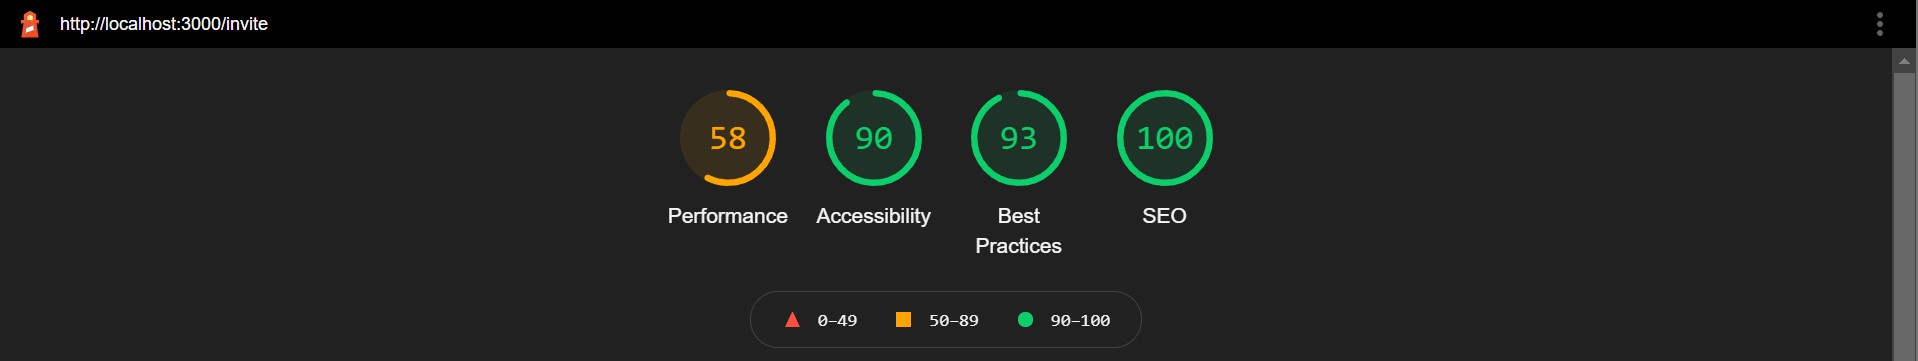
\includegraphics[scale=0.3]{images/accounts-student-lighthouse.jpg}
    \caption{Google Lighthouse Results for the Student Enrollment Dashboard}
\end{figure}
The student enrollment dashboard received near identical scores to the login and sign up page, with the same criticisms for each of the criteria. The accessibility score was a 90/100 due to some divs in the page that were used for styling not having the correct aria labels, and the performance was mostly impacted by non-minified JavaScript. Both of these can be easily rectified.

\textbf{Timeline}

Due to the interconnected nature of the staff and student enrollment features, the student features were completed on the same timeline ass the staff features. In the original timeline, this was broken out into standard and advanced enrollment features, with the standard features being manual enrollment and advanced being everything else. Standard features were planned on being completed in Week 9 of Term 2, and was completed on schedule. Advanced features were planned on being finished in Week 4 of Term 3, by which the code enrollment was completed, but the search functionality wasn't completed until week 7.

\textbf{Challenges Faced}

The primary challenge faced was creating an effective user-flow for both existing and new users to enroll using an invite code. It was found out very early during internal testing that although the invite codes worked very well for existing users, the process for a new user was less than ideal, as they would have to follow an invite link, then make an account, then re-enter the invite link in their browser. This process did not feel smooth and lead to a poor user experience. The solution was to implement a redirect system that allowed the login page to redirect to the student enrollment dashboard, if the link that took them to the login page was an invite link. This change greatly improved the new user experience.

Another challenge was the quality of search results returned to student users. Initially, the search only compared itself to course names and course codes, however it was found that this method did not help students who did not know the exact name of the course they were looking for, as it did not allow for more general searching. To fix this, the search was expanded to also search course outlines. This allows the search to be more powerful and give better results, however the cost is that the search takes a lot longer to complete. Although the time for search is a downside, it was decided that it was a worthwhile trade-off due to how much it improved the quality of the search results.